\subsubsection{Aufbau und Entwicklung des Frontends}  
\label{sec:Aufbau und Entwicklung des Frontends-1}

Durch eine zusätzliche Javascript-Bibliothek „Vue-resource“ werden asynchrone Anfragen an die Backend-\ac{API} geschickt, die die passenden Daten liefert. Um dem Nutzer ein wenig Arbeit abzunehmen werden sobald ein editierbares Feld verlassen wird die Daten auch in der Datenbank direkt aktualisiert. Vorausgesetzt es handelt sich um valide Daten.
Für jede Komponente wird das entsprechende Template anhand der ID definiert.
Die Daten werden anhand des data-Attributs festgelegt und können dann mithilfe von „this“ aufgerufen werden. 
Des Weiteren können auch Methoden definiert werden, welche dann aufgerufen werden können. Um eine Komponente mit Daten zu initialisieren wird die „created“-Eigenschaft verwendet. Diese wird sobald die Komponente erstellt wurde aufgerufen. Folgendes Codebeispiel zeigt die Komponente des Produkts. Wie man hier sieht wird sehr oft mit der \ac{REST}-\ac{API} kommuniziert.

\begin{lstlisting}[frame=single]
var product = Vue.component("product", {
  template: "#product",
  data: function () {
    return {
      product: new Product()
    };
  },
  methods: {
    saveProduct: function () {
      var url = api.products;
      this.$http.post(url, this.product).then(response => {
        this.product = new Product();
        $('#productModal').modal('hide');
        notie.alert({
          type: "success",
          text: "success",
          time: 1.5
        });
        this.$emit("save-product", response.body);
      }, response => {
        notie.alert({
          type: "error",
          text: response.statusText,
          time: 1.5
        });
      });
    }
  }
});
\end{lstlisting}

\clearpage

\subsubsection{Oberfläche}  
\label{sec:Oberfläche-1}

Folgend wird die Benutzeroberfläche anhand von Screenshots gezeigt. Es wurde großer Wert auf eine intuitive Bedienung gesetzt, deshalb sind die Komponenten auch so schlicht gestaltet worden.

\begin{figure}[!htb]
Der Warenkorb wird in Tabellenform dargestellt und aktualisiert sich bei jeder Änderung, die der Benutzer durchführt. Die Änderungen werden erst gespeichert, wenn der Benutzer auf den Save-Button drückt.	
  \begin{subfigure}{\linewidth}
	\centering
	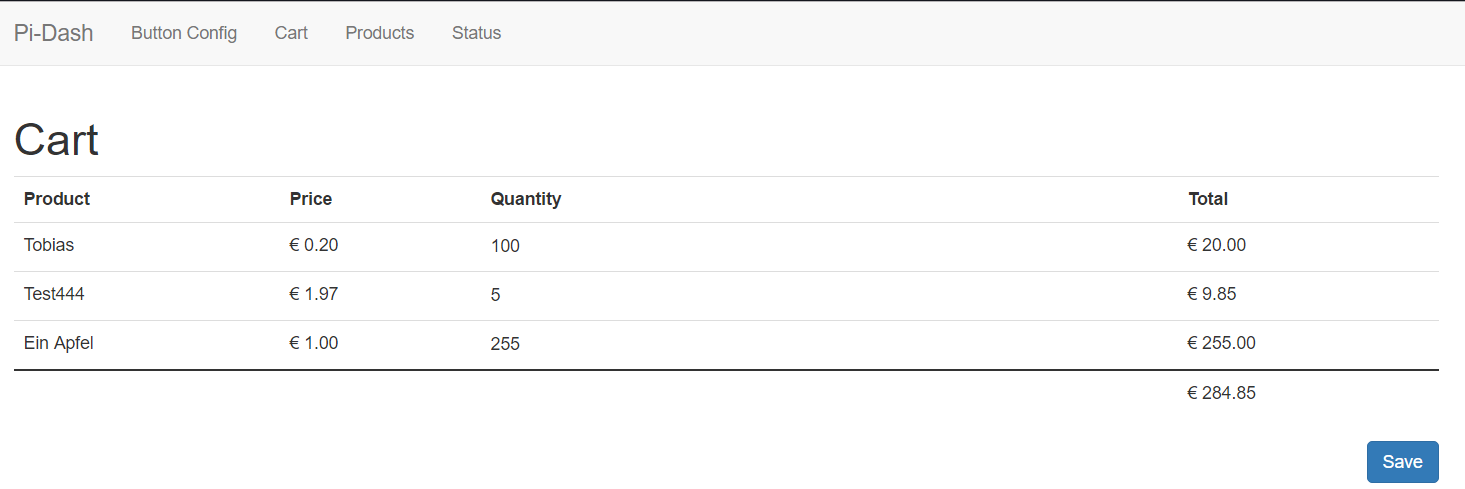
\includegraphics[scale=0.4]{Bilder/ui_cart.png}
	\caption[UI des Warenkorbs]{\ac{UI} des Warenkorbs}
  \end{subfigure}\par\medskip
  
Die Produkte aktualisieren sich, im Gegensatz zum Warenkorb, nach jeder Änderung, die der Benutzer gemacht hat. So muss der Benutzer nicht nach jeder Änderung extra auf einen Button drücken.

  \begin{subfigure}{\linewidth}	
	\centering
	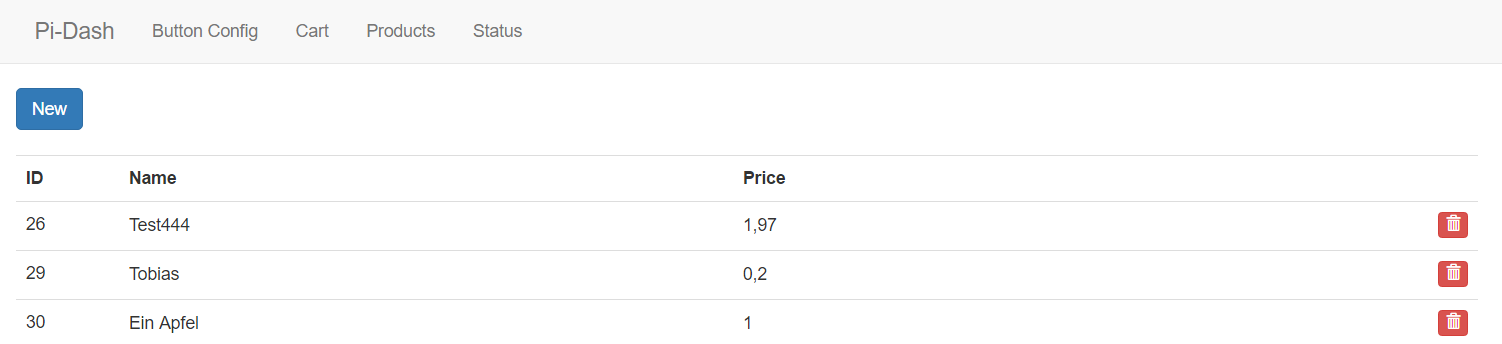
\includegraphics[scale=0.4]{Bilder/ui_products.png}
	\caption[UI der Produktübersicht]{\ac{UI} der Produktübersicht}
  \end{subfigure}\par\medskip
  
Die Statusübersicht der \ac{TCP}- und \ac{UDP}-Server besteht lediglich aus zwei Buttons, die je nach Status des Servers aktiv oder blockiert sind. Über diese können die Server, falls sie nicht aktiv sind gestartet werden.

  \begin{subfigure}{\linewidth}
	\centering
	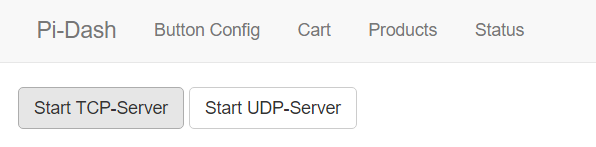
\includegraphics[scale=0.8]{Bilder/ui_status.png}
	\caption[UI der Statusseite]{\ac{UI} der Statusseite}
  \end{subfigure}
  \caption{User Interface,\\ Quelle: Eigene Aufnahmen}
\end{figure}

